\documentclass[11pt]{article}

\usepackage[a4paper,margin=1in]{geometry}
\usepackage{amsmath,amssymb}
\usepackage{booktabs}
\usepackage{graphicx}
\usepackage{hyperref}
\usepackage{siunitx}
\usepackage{tabularx}

\title{Methodology and Experimental Analysis of the Hamiltonian Vision Kernel}
\author{Sparsho Chakraborty}
\date{}

\begin{document}
\maketitle

\begin{abstract}
This work presents a methodological and experimental analysis of two Hamiltonian Vision Kernel (HVK) variants for image reconstruction. The first variant, denoted 1D HVK, uses a one-dimensional anisotropic Heisenberg Hamiltonian over nearest-neighbor qubit correlations. The second variant, denoted 2D HVK, extends the same reconstruction framework to a two-dimensional qubit-grid Hamiltonian. In both cases, an image is decomposed into tensor-network patch features, augmented with Fourier positional information, processed through a variational quantum circuit, and decoded back into pixel space. The resulting training curves, reconstruction tables, order-parameter trajectories, and static phase-transition snapshots indicate that the learned Hamiltonian acts as a physically motivated regularizer for image reconstruction. The comparison further shows that the 2D HVK improves reconstruction error and reaches a lower Hamiltonian energy on the present benchmark.
\end{abstract}

\section{Dataset and Preprocessing}

The experiments use a single grayscale image dataset consisting of \texttt{monalisa.jpg}. The image is resized to $256 \times 256$ pixels and normalized to the range $[0,1]$. It is then partitioned into a regular grid of non-overlapping $64 \times 64$ patches. This produces
\begin{equation}
N = \left(\frac{256}{64}\right)^2 = 16
\end{equation}
image patches. Each patch $P_{ij} \in \mathbb{R}^{64 \times 64}$ is associated with its grid coordinate $(i,j)$, where $i,j \in \{0,1,2,3\}$.

Each patch is vectorized into a $4096$-dimensional vector. Since $4096 = 2^{12}$, the vector is interpreted as a twelve-site spin-$1/2$ quantum state. The normalized vector is reshaped as
\begin{equation}
|\psi\rangle \in \left(\mathbb{C}^{2}\right)^{\otimes 12},
\end{equation}
and compressed into a matrix product state (MPS) with maximum bond dimension $\chi=4$. The MPS representation is used to extract local Pauli expectation values, nearest-neighbor correlations, and bipartite entanglement entropies.

\section{MPS Feature Extraction}

For each patch, the MPS encoder computes three classes of quantum-inspired descriptors. First, local Pauli expectation values are evaluated at each of the twelve tensor sites:
\begin{equation}
\langle Z_i\rangle = \langle \psi | Z_i | \psi \rangle,
\qquad
\langle X_i\rangle = \langle \psi | X_i | \psi \rangle.
\end{equation}
This gives $24$ local features. Second, nearest-neighbor $ZZ$ correlations are computed as
\begin{equation}
\langle Z_i Z_{i+1}\rangle
= \langle \psi | Z_i Z_{i+1} | \psi \rangle,
\qquad i=0,\ldots,10,
\end{equation}
which contributes $11$ correlation features. Third, the Schmidt spectrum at each internal bond is used to compute the bipartite entropy
\begin{equation}
S_i = -\sum_k p_k^{(i)} \log \left(p_k^{(i)} + \epsilon\right),
\end{equation}
where $p_k^{(i)}$ are normalized squared Schmidt coefficients and $\epsilon=10^{-8}$ is used for numerical stability. These $11$ entropy features encode the distribution of entanglement across the patch.

The complete feature vector for each patch is therefore
\begin{equation}
f_n =
\left[
\langle Z_i\rangle,
\langle X_i\rangle,
\langle Z_i Z_{i+1}\rangle,
S_i
\right]
\in \mathbb{R}^{46}.
\end{equation}
Across the $16$ patches, the feature matrix $F \in \mathbb{R}^{16 \times 46}$ is standardized to zero mean and unit variance per feature dimension before being passed to the quantum model.

\section{Spatial Positional Encoding}

The MPS representation captures patch content, but it does not by itself encode where the patch belongs in the image. Therefore, each patch coordinate is mapped into an $8$-dimensional sinusoidal positional encoding. For normalized row and column coordinates $(r,c)$, the encoding contains sine and cosine components at multiple frequencies:
\begin{equation}
e(r,c) =
\left[
\sin(\omega_k \pi r),
\cos(\omega_k \pi r),
\sin(\omega_k \pi c),
\cos(\omega_k \pi c)
\right]_{k=0}^{1}
\in \mathbb{R}^{8}.
\end{equation}
This positional vector is projected into six learned rotation angles and injected into the variational quantum circuit through per-qubit $RY$ rotations. As a result, two patches with similar MPS features but different spatial coordinates can still produce distinct quantum observable vectors.

\section{1D HVK: One-Dimensional Hamiltonian Formulation}

The 1D HVK implements a chain-structured Hamiltonian Vision Kernel. The standardized MPS feature vector is projected into a six-dimensional quantum input and embedded into a six-qubit PennyLane circuit. The circuit uses two variational layers and produces a $27$-dimensional observable vector containing local $Z$ and $X$ expectations together with nearest-neighbor $ZZ$, $XX$, and $YY$ correlations:
\begin{equation}
o_n =
\left[
\langle Z_i\rangle,
\langle X_i\rangle,
\langle Z_iZ_{i+1}\rangle,
\langle X_iX_{i+1}\rangle,
\langle Y_iY_{i+1}\rangle
\right]
\in \mathbb{R}^{27}.
\end{equation}

The Hamiltonian energy is defined using learnable anisotropic Heisenberg couplings:
\begin{equation}
E_n =
\sum_{i=0}^{4}
\left(
J_z^{(i)}\langle Z_iZ_{i+1}\rangle_n
+ J_x^{(i)}\langle X_iX_{i+1}\rangle_n
+ J_y^{(i)}\langle Y_iY_{i+1}\rangle_n
\right).
\end{equation}
The learnable parameters $J_x$, $J_y$, and $J_z$ allow the Hamiltonian to adapt to the image statistics rather than enforcing a fixed physical prior.

For the 1D HVK, the order-parameter sector is computed directly from the same observable vector used by the Hamiltonian. Let $Z_{n,q,t}$ and $X_{n,q,t}$ denote the measured local Pauli expectations for patch $n$, qubit $q$, and epoch $t$:
\begin{equation}
Z_{n,q,t}=\langle Z_q\rangle_{n,t},
\qquad
X_{n,q,t}=\langle X_q\rangle_{n,t}.
\end{equation}
The patch-wise longitudinal and transverse magnetizations are
\begin{equation}
m_{n,t}^{z,1D}
=
\frac{1}{Q}
\sum_{q=1}^{Q} Z_{n,q,t},
\qquad
m_{n,t}^{x,1D}
=
\frac{1}{Q}
\sum_{q=1}^{Q} X_{n,q,t},
\qquad Q=6.
\end{equation}
The global 1D order parameters recorded at epoch $t$ are therefore
\begin{equation}
m_t^{z,1D}
=
\frac{1}{N}\sum_{n=1}^{N}m_{n,t}^{z,1D},
\qquad
|m|_t^{1D}
=
\frac{1}{N}\sum_{n=1}^{N}\left|m_{n,t}^{z,1D}\right|,
\qquad
m_t^{x,1D}
=
\frac{1}{N}\sum_{n=1}^{N}m_{n,t}^{x,1D}.
\end{equation}
The 1D lattice-correlation order statistic includes all three anisotropic Heisenberg channels:
\begin{equation}
C_t^{1D}
=
\frac{1}{3NB}
\sum_{n=1}^{N}
\sum_{i=0}^{B-1}
\left(
\langle Z_iZ_{i+1}\rangle_{n,t}
+\langle X_iX_{i+1}\rangle_{n,t}
+\langle Y_iY_{i+1}\rangle_{n,t}
\right),
\qquad B=5.
\end{equation}
Thus, the 1D HVK tracks not only the reconstruction loss and mean Hamiltonian energy, but also the longitudinal magnetization, transverse magnetization, absolute magnetization, and full anisotropic correlator alignment induced by the learned Heisenberg chain.

The decoder is a multilayer perceptron that receives the observable vector concatenated with the positional encoding and outputs a reconstructed $64 \times 64$ patch. The complete image is reconstructed by stitching the predicted patches and applying seam blending.

\begin{figure}[t]
\centering
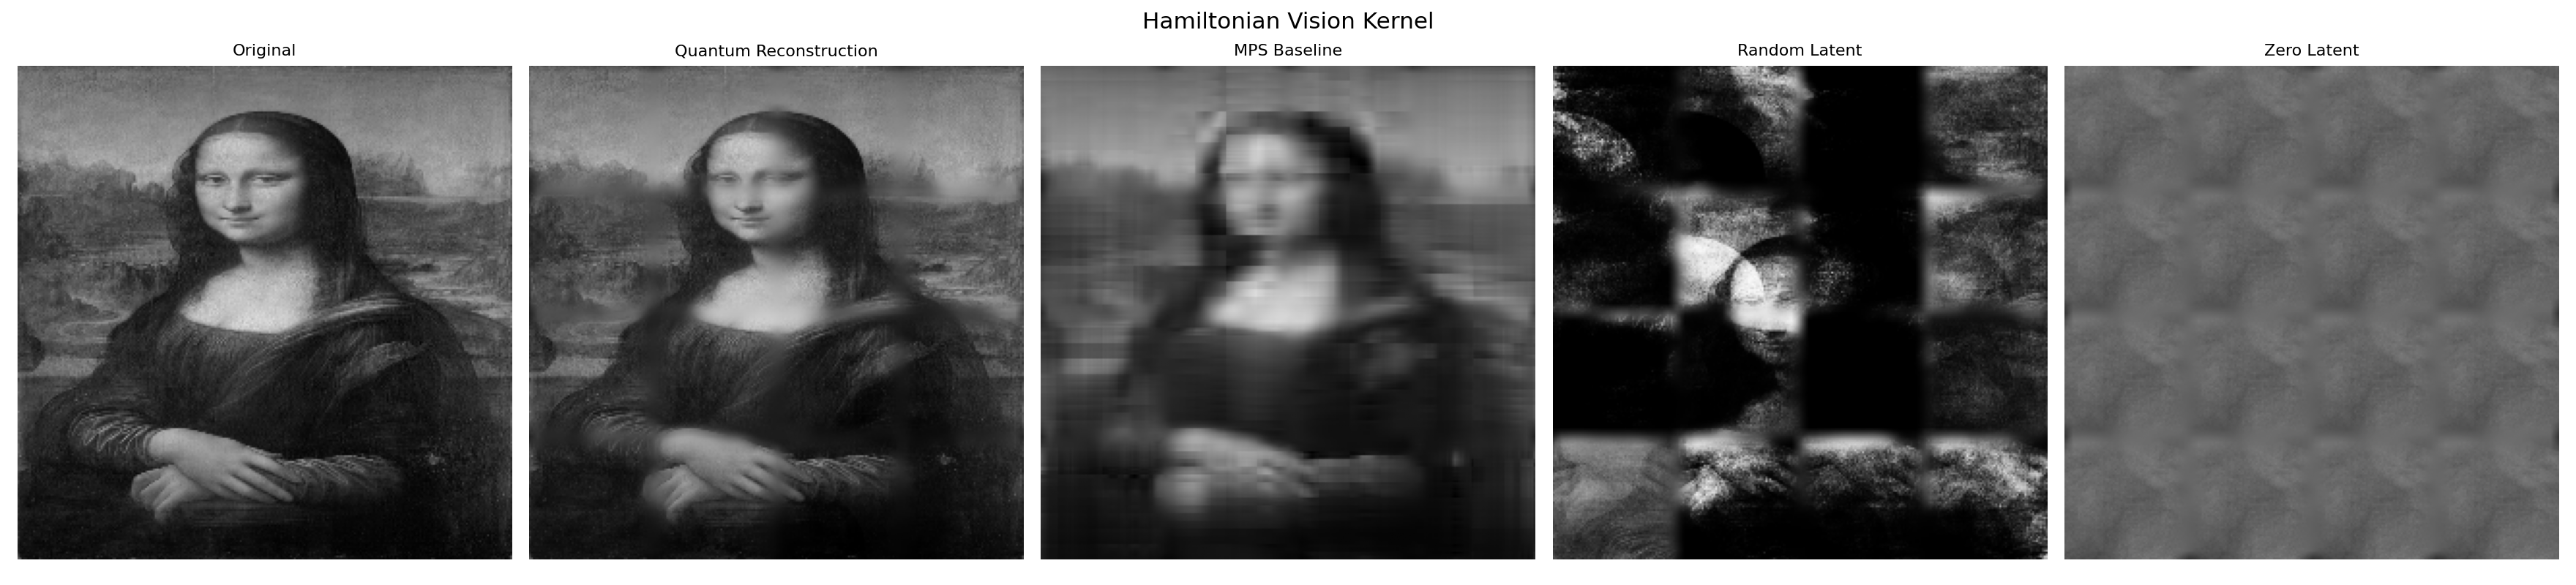
\includegraphics[width=0.95\linewidth]{Main/outputs/training_analysis/reconstructions.png}
\caption{Static reconstruction comparison for the 1D HVK experiment. The panels compare the input image, the HVK reconstruction, the tensor-network MPS baseline, and decoder outputs under random and zero latent controls.}
\label{fig:1d_recon}
\end{figure}

\section{2D HVK: Two-Dimensional Hamiltonian Formulation}

The 2D HVK extends the model from a one-dimensional nearest-neighbor chain to a two-dimensional qubit lattice. The circuit still uses six qubits, but they are arranged as a $2 \times 3$ grid. The graph contains four horizontal edges and three vertical edges:
\begin{equation}
\mathcal{E}_h = \{(0,1),(1,2),(3,4),(4,5)\},
\qquad
\mathcal{E}_v = \{(0,3),(1,4),(2,5)\}.
\end{equation}
The model returns local $Z$ expectations, local $X$ expectations, and all $ZZ$ correlations over the two-dimensional edge set. Therefore, the 2D HVK observable vector has dimension
\begin{equation}
6 + 6 + 7 = 19.
\end{equation}

The 2D HVK Hamiltonian energy is
\begin{equation}
E_n^{2D} =
\sum_{(u,v)\in \mathcal{E}_h \cup \mathcal{E}_v}
J_{uv}\langle Z_uZ_v\rangle_n,
\end{equation}
where the edge couplings $J_{uv}$ are learned jointly with the circuit and decoder. This formulation directly models horizontal and vertical lattice correlations, making the 2D HVK closer to the spatial geometry of the image patch grid.

The order-parameter sector for the 2D HVK is defined analogously, but its correlation statistic is evaluated on the two-dimensional qubit edge set. For local observables
\begin{equation}
Z_{n,q,t}^{2D}=\langle Z_q\rangle_{n,t},
\qquad
X_{n,q,t}^{2D}=\langle X_q\rangle_{n,t},
\end{equation}
the patch-wise longitudinal and transverse order parameters are
\begin{equation}
m_{n,t}^{z,2D}
=
\frac{1}{Q}
\sum_{q=1}^{Q}Z_{n,q,t}^{2D},
\qquad
m_{n,t}^{x,2D}
=
\frac{1}{Q}
\sum_{q=1}^{Q}X_{n,q,t}^{2D}.
\end{equation}
The corresponding epoch-level observables are
\begin{equation}
m_t^{z,2D}
=
\frac{1}{N}\sum_{n=1}^{N}m_{n,t}^{z,2D},
\qquad
|m|_t^{2D}
=
\frac{1}{N}\sum_{n=1}^{N}\left|m_{n,t}^{z,2D}\right|,
\qquad
m_t^{x,2D}
=
\frac{1}{N}\sum_{n=1}^{N}m_{n,t}^{x,2D}.
\end{equation}
Since the 2D HVK Hamiltonian uses the spatial edge set $\mathcal{E}$, its lattice-correlation order statistic is
\begin{equation}
C_t^{2D}
=
\frac{1}{N|\mathcal{E}|}
\sum_{n=1}^{N}
\sum_{(u,v)\in\mathcal{E}}
\langle Z_uZ_v\rangle_{n,t},
\qquad
|\mathcal{E}|=7.
\end{equation}
The 2D order sector therefore measures the same longitudinal and transverse spin alignment as the 1D HVK, but replaces the one-dimensional anisotropic bond average with a geometric average over horizontal and vertical qubit-grid interactions.

\section{Symmetry Discretization from Spin Rotations to the Square Patch Group}

The HVK latent representation may be viewed as a field of quantum observable vectors over the image patch lattice. Before positional modulation, the local qubit state generated by the variational circuit belongs to the projective Hilbert space
\begin{equation}
|\Psi_n\rangle \in \mathbb{CP}^{2^Q-1}=\mathbb{CP}^{63},
\qquad Q=6,
\end{equation}
and the local spin expectation vector
\begin{equation}
\mathbf{s}_{n,q}
=
\left(
\langle X_q\rangle_n,
\langle Y_q\rangle_n,
\langle Z_q\rangle_n
\right)
\in \mathbb{R}^{3}
\end{equation}
transforms under the adjoint action of $SU(2)$ as
\begin{equation}
U\in SU(2):
\qquad
\mathbf{s}_{n,q}\mapsto R(U)\mathbf{s}_{n,q},
\qquad
R(U)\in SO(3).
\end{equation}
In the isotropic Heisenberg limit, the interaction
\begin{equation}
H_{\mathrm{iso}}
=
J\sum_{(u,v)\in\mathcal{E}}
\left(
X_uX_v+Y_uY_v+Z_uZ_v
\right)
\end{equation}
is invariant under global $SU(2)$ spin rotations. The learned anisotropic couplings and the restricted observable sectors break this exact invariance, but the latent correlator geometry remains organized by the $SU(2)$ spin-action structure.

The reduction from continuous spin symmetry to discrete image symmetry occurs through the positional field. Each patch coordinate $p=(i,j)$ is mapped to a Fourier feature $e(p)$ and then to learned qubit angles
\begin{equation}
\theta_{\mathrm{pos}}(p)=W_{\mathrm{pos}}e(p)\in\mathbb{R}^{Q}.
\end{equation}
The patch-dependent circuit state is therefore
\begin{equation}
|\Psi_{p}\rangle
=
U_{\mathrm{var}}(\theta)
U_{\mathrm{pos}}\!\left(\theta_{\mathrm{pos}}(p)\right)
U_{\mathrm{enc}}\!\left(W_f f_p\right)
|0\rangle^{\otimes Q}.
\end{equation}
Because $\theta_{\mathrm{pos}}(p)$ depends explicitly on the grid coordinate, arbitrary patch permutations are no longer symmetries of the representation. The only geometric transformations that preserve the square patch lattice are the elements of the dihedral group
\begin{equation}
D_4
=
\langle r,s \mid r^4=e,\; s^2=e,\; srs=r^{-1}\rangle,
\end{equation}
where $r$ is a $90^\circ$ rotation and $s$ is a reflection.

Let $\Lambda=\{0,1,2,3\}^2$ denote the $4\times4$ patch lattice. The dihedral group acts on patch coordinates as
\begin{equation}
g:\Lambda\rightarrow\Lambda,
\qquad g\in D_4.
\end{equation}
The HVK observable field is the map
\begin{equation}
\mathcal{O}_A:\Lambda\rightarrow\mathbb{R}^{d_A},
\qquad
p\mapsto o_p^A,
\qquad
d_{1D}=27,\quad d_{2D}=19.
\end{equation}
Under a square-lattice symmetry $g\in D_4$, the ideal equivariant transformation has the form
\begin{equation}
\mathcal{O}_A(gp)
\approx
\rho_A(g)\mathcal{O}_A(p),
\qquad
\rho_A(g)\in O(d_A),
\end{equation}
where $\rho_A$ is the induced representation on the observable coordinates. This is the precise sense in which the continuous $SU(2)$ spin-rotation organization is discretized into a $D_4$-structured image-lattice representation.

For the 1D HVK, the internal Hamiltonian graph is a qubit chain, so $D_4$ does not arise from the qubit interaction graph itself. Instead, it arises from the image-domain patch lattice through the positional encoding. The chain Hamiltonian supplies anisotropic spin-correlation channels $(ZZ,XX,YY)$, while the square positional field assigns those channels to a $D_4$-organized set of image locations:
\begin{equation}
\left\{
o_{(i,j)}^{1D}
\right\}_{(i,j)\in\Lambda}
\quad\text{with}\quad
\Lambda/D_4
\text{ defining the square-grid symmetry classes.}
\end{equation}
For the 2D HVK, the observable field is also indexed by the same square patch lattice, but the Hamiltonian itself contains horizontal and vertical qubit-grid edges. Consequently, the 2D HVK has a stronger spatial inductive bias: both the patch-position field and the internal correlation graph distinguish lattice directions. The resulting discretization can be summarized as
\begin{align}
SU(2)\;\text{spin action}
&\xrightarrow{\;\theta_{\mathrm{pos}}(i,j)\;}
\text{position-conditioned observable field}
\nonumber\\
&\xrightarrow{\;\Lambda=\{0,1,2,3\}^2\;}
D_4\;\text{square-lattice organization}.
\end{align}
This construction does not claim that the trained finite model has exact $D_4$ equivariance. Rather, $D_4$ is the residual geometric symmetry group of the discretized image lattice after continuous spin and permutation degeneracies are broken by positional modulation.

\section{Training Objective}

Both pipelines optimize a hybrid reconstruction-energy objective. Given a decoder $D(\cdot)$, observable vector $o_n$, positional encoding $e_n$, and target patch $P_n$, the reconstruction loss is
\begin{equation}
\mathcal{L}_{rec}
=
\frac{1}{N}
\sum_{n=1}^{N}
\left\|
D(o_n,e_n) - P_n
\right\|_F^2.
\end{equation}
The energy loss is the mean Hamiltonian energy across patches:
\begin{equation}
\mathcal{L}_{energy}
=
\frac{1}{N}
\sum_{n=1}^{N} E_n.
\end{equation}
The final objective is
\begin{equation}
\mathcal{L}_{total}
=
\mathcal{L}_{rec}
+ \lambda \mathcal{L}_{energy},
\qquad
\lambda = 0.01.
\end{equation}
This objective trains the decoder to preserve image structure while encouraging the quantum latent state to move toward low-energy correlated configurations.

\begin{figure}[t]
\centering
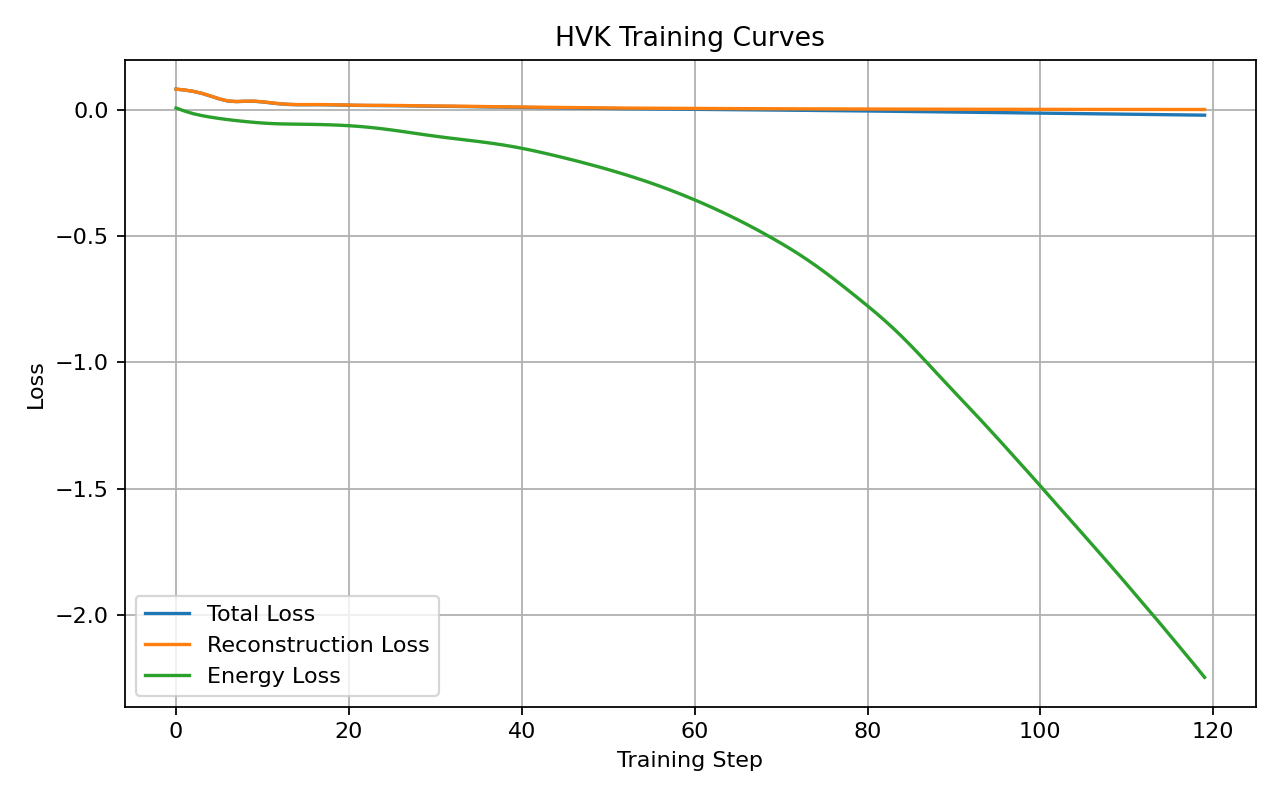
\includegraphics[width=0.82\linewidth]{Main/outputs/training_analysis/training_curves.png}
\caption{Training curves for the 1D HVK, showing the reconstruction term, Hamiltonian energy term, and total objective over optimization.}
\label{fig:1d_training}
\end{figure}

\section{Order Parameters and Phase-Transition Detection}

During training, the model records both patch-level and epoch-level observables. The order parameter is computed from the longitudinal magnetization of the learned quantum observable state. For patch $n$ at training epoch $t$, the patch-wise longitudinal order parameter is defined as
\begin{equation}
m_{n,t}^{(z)}
=
\frac{1}{Q}
\sum_{q=1}^{Q}
\langle Z_q\rangle_{n,t},
\end{equation}
where $Q=6$ is the number of qubits and $\langle Z_q\rangle_{n,t}$ is the local Pauli-$Z$ expectation value of qubit $q$ for patch $n$. The epoch-level order parameter is then obtained by averaging over all $N=16$ patches:
\begin{equation}
m_t =
\frac{1}{N}
\sum_{n=1}^{N}
\;m_{n,t}^{(z)}
=
\frac{1}{NQ}
\sum_{n=1}^{N}
\sum_{q=1}^{Q}
\langle Z_q\rangle_{n,t}.
\end{equation}
This scalar tracks the global alignment of the learned latent spin configuration along the $Z$ axis.

The absolute order parameter is computed as
\begin{equation}
|m|_t =
\frac{1}{N}
\sum_{n=1}^{N}
\left|m_{n,t}^{(z)}\right|,
\end{equation}
which measures the strength of ordering independently of sign. The transverse order parameter is computed from local $X$ expectations:
\begin{equation}
m_t^{(x)}
=
\frac{1}{NQ}
\sum_{n=1}^{N}
\sum_{q=1}^{Q}
\langle X_q\rangle_{n,t}.
\end{equation}
The lattice-correlation statistic differs between the two variants. For the 1D HVK, the recorded total lattice correlation is the average of the nearest-neighbor $ZZ$, $XX$, and $YY$ correlator sectors:
\begin{equation}
C_t^{1D}
=
\frac{1}{3N}
\sum_{n=1}^{N}
\left[
\overline{ZZ}_{n,t}
+ \overline{XX}_{n,t}
+ \overline{YY}_{n,t}
\right],
\end{equation}
where each bar denotes the mean over the five nearest-neighbor bonds in that sector. For the 2D HVK, the lattice-correlation statistic is the mean $ZZ$ correlation over the two-dimensional edge set:
\begin{equation}
C_t^{2D}
=
\frac{1}{N|\mathcal{E}|}
\sum_{n=1}^{N}
\sum_{(u,v)\in \mathcal{E}}
\langle Z_u Z_v\rangle_{n,t},
\qquad
\mathcal{E}=\mathcal{E}_h\cup\mathcal{E}_v.
\end{equation}
Mean Hamiltonian energy is recorded separately as the average patch energy at epoch $t$.

A susceptibility-like signal is computed from the epoch-to-epoch change in the mean order parameter:
\begin{equation}
\chi_t = |m_t - m_{t-1}|.
\end{equation}
A phase transition is detected when the maximum susceptibility exceeds a threshold defined by
\begin{equation}
\tau = \operatorname{median}(\chi) + 2\sigma_\chi.
\end{equation}
This rule identifies abrupt reorganizations in the learned observable manifold during training. In this sense, the detected critical epoch is not treated as a thermodynamic phase transition in the strict infinite-system limit; rather, it is used as a finite-size diagnostic of rapid latent-state reorganization during optimization.

\begin{figure}[t]
\centering
\begin{minipage}{0.48\linewidth}
\centering

\includegraphics[width=\linewidth]{Main/outputs/training_analysis/hvk_order_parameter_curve.png}
\end{minipage}
\hfill
\begin{minipage}{0.48\linewidth}
\centering
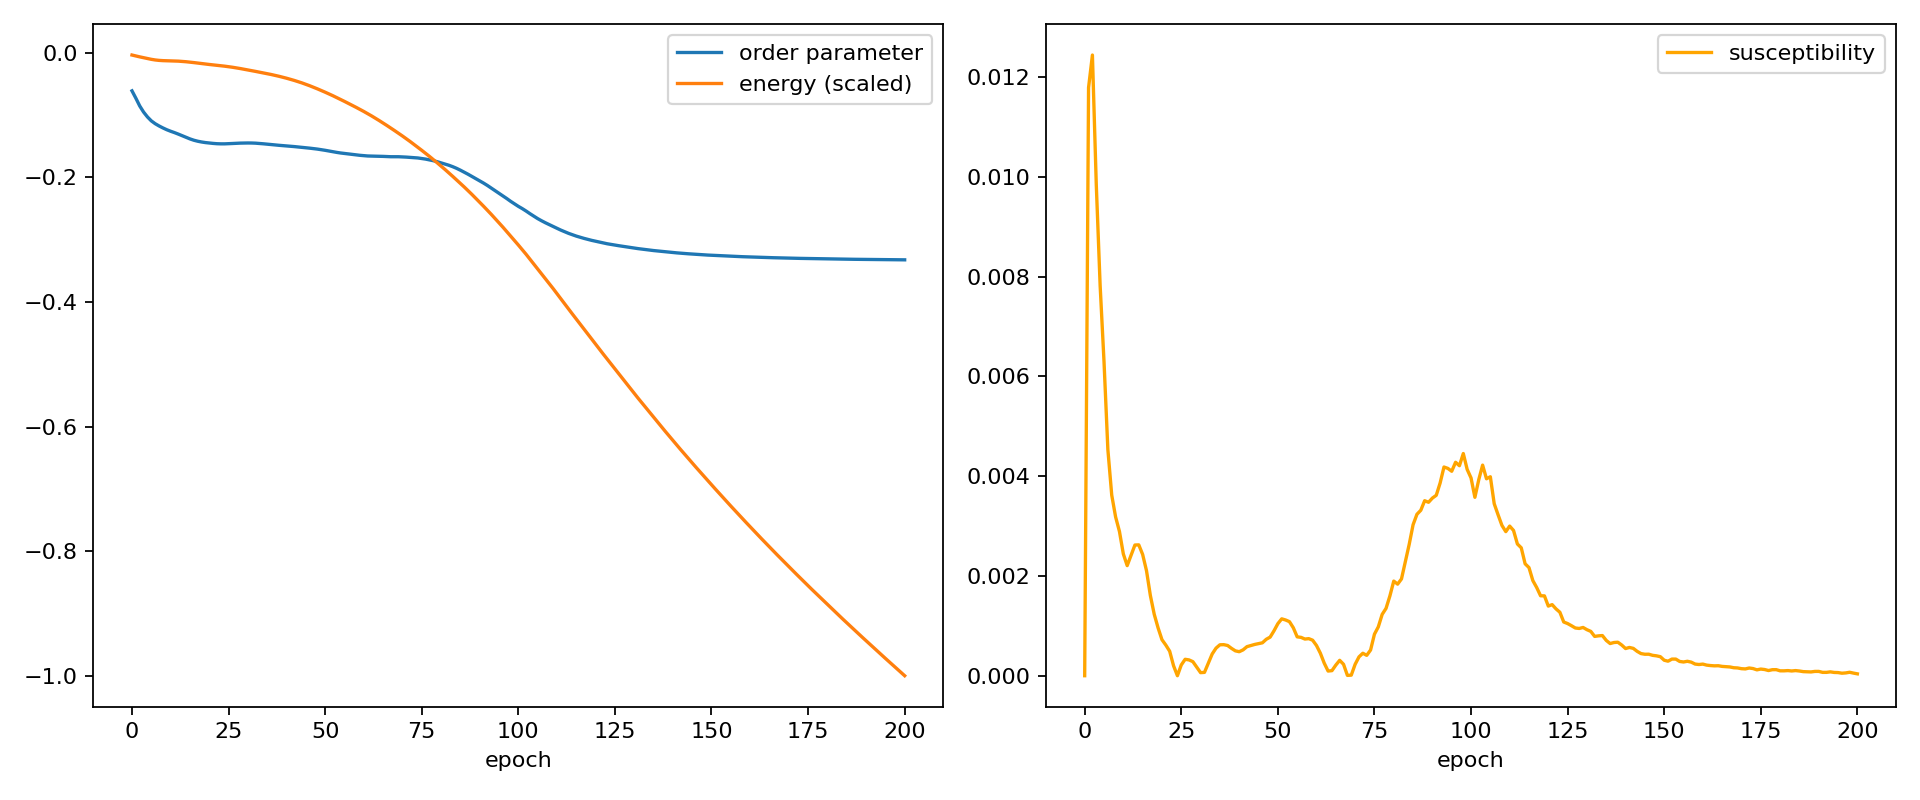
\includegraphics[width=\linewidth]{Main2/outputs/training_analysis/hvk_order_parameter_curve.png}
\end{minipage}
\caption{Order-parameter trajectories for the 1D HVK and 2D HVK experiments. The susceptibility criterion is applied to each epoch-wise signal to identify the corresponding finite-size critical reorganization point.}
\label{fig:order_curves}
\end{figure}

\section{Experimental Setup}

\begin{table}[h]
\centering
\caption{Training configuration used in the recent HVK runs.}
\begin{tabular}{lll}
\toprule
Parameter & 1D HVK & 2D HVK \\
\midrule
Input image & \texttt{monalisa.jpg} & \texttt{monalisa.jpg} \\
Image size & $256 \times 256$ & $256 \times 256$ \\
Patch size & $64 \times 64$ & $64 \times 64$ \\
Number of patches & $16$ & $16$ \\
MPS sites & $12$ & $12$ \\
MPS bond dimension & $4$ & $4$ \\
MPS feature dimension & $46$ & $46$ \\
Positional dimension & $8$ & $8$ \\
Qubits & $6$ & $6$ \\
Circuit layers & $2$ & $2$ \\
Observable dimension & $27$ & $19$ \\
Learning rate & $0.003$ & $0.004$ \\
Recorded epochs & $0$--$199$ & $0$--$200$ \\
Optimizer & Adam & Adam \\
\bottomrule
\end{tabular}
\end{table}

\section{Results, Benchmarks, and Comparative Analysis}

The outputs were saved as static reconstruction frames, training tables, order-parameter plots, and patch-level correlation tables. The 1D HVK produced reconstruction images, a tensor-network MPS baseline, random-latent and zero-latent reconstructions, observable maps, entropy maps, and training curves. The 2D HVK produced epoch-wise reconstruction frames, the order-parameter curve, and patch-level lattice-correlation tables. Only static PNG outputs are used for paper reporting.

For a model variant $A \in \{\mathrm{1D},\mathrm{2D}\}$ and epoch $t$, the empirical reconstruction benchmark is the patch-averaged mean-squared error
\begin{equation}
\operatorname{MSE}_{A}(t)
=
\frac{1}{N}
\sum_{n=1}^{N}
\frac{1}{64^2}
\left\|
\widehat{P}_{n,t}^{A} - P_n
\right\|_F^2,
\end{equation}
where $P_n$ is the target patch and $\widehat{P}_{n,t}^{A}$ is the decoded patch. The best reconstruction epoch is
\begin{equation}
t_A^{\star} =
\arg\min_t \operatorname{MSE}_{A}(t),
\qquad
\operatorname{MSE}_{A}^{\star}
=
\min_t \operatorname{MSE}_{A}(t).
\end{equation}
The relative final-error improvement of the 2D HVK over the 1D HVK is measured as
\begin{equation}
\Delta_{\mathrm{MSE}}
=
\frac{
\operatorname{MSE}_{\mathrm{1D}}(T_{\mathrm{1D}})
-
\operatorname{MSE}_{\mathrm{2D}}(T_{\mathrm{2D}})
}{
\operatorname{MSE}_{\mathrm{1D}}(T_{\mathrm{1D}})
}
\times 100\%.
\end{equation}
Using the recorded final epochs, this gives $\Delta_{\mathrm{MSE}}\approx 74.8\%$.

The Hamiltonian descent is quantified by
\begin{equation}
\Delta E_A =
\overline{E}_A(T_A)-\overline{E}_A(0),
\qquad
\overline{E}_A(t)=\frac{1}{N}\sum_{n=1}^{N}E_{n,t}^{A}.
\end{equation}
This quantity is not interpreted as an absolute physical energy across different Hamiltonian graphs; instead, it measures how strongly each model moves toward its own learned low-energy latent configuration.

\begin{table}[h]
\centering
\caption{Quantitative benchmark summary from the saved training outputs.}
\begin{tabular}{lcc}
\toprule
Metric & 1D HVK & 2D HVK \\
\midrule
Initial reconstruction MSE & $8.1035\times 10^{-2}$ & $8.1095\times 10^{-2}$ \\
Final reconstruction MSE & $3.3741\times 10^{-4}$ & $8.5149\times 10^{-5}$ \\
Best reconstruction MSE & $1.9283\times 10^{-4}$ & $8.4902\times 10^{-5}$ \\
Best-MSE epoch & $181$ & $199$ \\
Initial total loss & $8.1346\times 10^{-2}$ & $8.0953\times 10^{-2}$ \\
Final total loss & $-3.6873\times 10^{-2}$ & $-7.0034\times 10^{-2}$ \\
Initial mean energy & $2.2166\times 10^{-2}$ & $-2.5700\times 10^{-2}$ \\
Final mean energy & $-3.7821$ & $-7.0510$ \\
Initial order parameter & $-6.3847\times 10^{-2}$ & $-6.1133\times 10^{-2}$ \\
Final order parameter & $-3.8271\times 10^{-3}$ & $-3.3240\times 10^{-1}$ \\
Detected critical epoch & $11$ & $2$ \\
Maximum susceptibility & $2.3162\times 10^{-3}$ & $1.2439\times 10^{-2}$ \\
Final-error reduction from initial MSE & $99.58\%$ & $99.90\%$ \\
\bottomrule
\end{tabular}
\end{table}

The benchmark results show that both HVK variants substantially reduce reconstruction error over training. The 1D HVK reaches a final reconstruction MSE of $3.3741\times 10^{-4}$ after $200$ recorded epochs, with its best reconstruction at epoch $181$. The 2D HVK reaches a lower final reconstruction MSE of $8.5149\times 10^{-5}$, with its best reconstruction at epoch $199$. Relative to the 1D HVK final MSE, the 2D HVK reduces the final reconstruction error by approximately $74.8\%$. This indicates that the two-dimensional Hamiltonian coupling structure provides a stronger spatial inductive bias for the present image reconstruction benchmark.

The energy trajectories also differ between the two models. The 1D HVK decreases the mean Hamiltonian energy from $2.2166\times 10^{-2}$ to $-3.7821$, while the 2D HVK decreases it from $-2.5700\times 10^{-2}$ to $-7.0510$. The stronger negative energy reached by the 2D HVK suggests that the two-dimensional lattice Hamiltonian learns a more strongly correlated low-energy representation under the same reconstruction task.

Both models exhibit a detected susceptibility peak. The 1D HVK detects a phase-transition-like event at epoch $11$, where the susceptibility peak exceeds the median-plus-two-standard-deviation threshold. The 2D HVK detects a sharper early transition at epoch $2$, with a larger maximum susceptibility. In the output visualizations, this transition corresponds to the period where the reconstructed image rapidly moves from a poorly organized latent representation toward a structured reconstruction.

Overall, the comparison suggests that the 2D HVK improves the reconstruction benchmark by aligning the Hamiltonian interaction graph with the spatial structure of image patches. The 1D HVK remains useful as a controlled chain-based baseline because it includes the full anisotropic $ZZ$, $XX$, and $YY$ correlator sectors. The 2D HVK, in contrast, emphasizes spatially organized $ZZ$ interactions over horizontal and vertical edges, which appears to produce stronger low-energy organization and lower reconstruction error in the present experiment.

\subsection{Benchmark Extension Against PHL and GAN Baselines}

The repository now contains measured runs for the 1D HVK in \texttt{Main}, the 2D HVK in \texttt{Main2}, and two independent baselines under \texttt{Baselines}: a Parameterized Hamiltonian Learning (PHL) segmentation baseline and a GAN reconstruction baseline. The PHL baseline was evaluated against an Otsu pseudo-mask because the present image experiment does not include a manually annotated segmentation mask. The GAN baseline was evaluated on the same \texttt{monalisa.jpg} reconstruction task using the same $256\times256$ image size and $64\times64$ patch scale. Additionally, to evaluate generalization, the 1D HVK and GAN baselines were evaluated on a CIFAR-10 test subset consisting of 10 images of size $32\times32$, with their average performance metrics reported.

PHL and HVK are related because both use Hamiltonian structure, but they optimize different objects. In the PHL image-segmentation baseline, the Hamiltonian parameters are learned so that the resulting energy landscape separates image regions into a binary mask. The output is a mask or probability field, and the natural metrics are Dice score, intersection-over-union (IoU), boundary F-score, and pixel accuracy. In HVK, the Hamiltonian is not the segmentation model itself. It acts as a latent physical regularizer inside an autoencoding pipeline: MPS patch features and positional encodings are transformed by a variational circuit, decoded back into image patches, and trained with reconstruction loss plus Hamiltonian energy. The natural HVK metrics are reconstruction MSE, PSNR/SSIM, Hamiltonian energy descent, order-parameter movement, and susceptibility peaks.

A GAN benchmark should also be interpreted differently from PHL. A GAN adds a discriminator that scores whether reconstructed patches look realistic. This can improve perceptual sharpness, but it does not directly provide a Hamiltonian energy or phase-transition diagnostic. The present GAN baseline reports MSE, PSNR, and SSIM; LPIPS and FID should be added only when a larger dataset is available. A hybrid HVK--GAN experiment would keep the HVK encoder/Hamiltonian path and add an adversarial image-space loss:
\begin{equation}
\mathcal{L}_{\mathrm{HVK\text{-}GAN}}
=
\mathcal{L}_{\mathrm{rec}}
+ \lambda_E \overline{E}
+ \lambda_{\mathrm{adv}}\mathcal{L}_{\mathrm{adv}},
\end{equation}
where $\mathcal{L}_{\mathrm{rec}}$ measures patch reconstruction, $\overline{E}$ is the learned Hamiltonian energy, and $\mathcal{L}_{\mathrm{adv}}$ is supplied by the discriminator.

\begin{table}[h]
\centering
\caption{Measured metric summary for HVK, PHL, and GAN baselines. The CIFAR-10 subset rows use images drawn from the CIFAR-10 dataset~\cite{krizhevsky2009learning}. Reconstruction metrics use normalized pixel intensities, so lower MSE and higher PSNR/SSIM are better.}
\label{tab:phl_gan_benchmark}
\small
\setlength{\tabcolsep}{3pt}
\begin{tabular}{lcccccccc}
\toprule
Model & Final MSE & Best MSE & PSNR & SSIM & Energy & Critical epoch & Dice & IoU \\
\midrule
\multicolumn{9}{l}{\textit{Monalisa Image Reconstruction}} \\
1D HVK & $3.3741\times10^{-4}$ & $1.9283\times10^{-4}$ & $34.72$ & -- & $-3.7821$ & $11$ & -- & -- \\
2D HVK & $8.5149\times10^{-5}$ & $8.4902\times10^{-5}$ & $40.70$ & -- & $-7.0510$ & $2$ & -- & -- \\
GAN & $1.0174\times10^{-3}$ & $9.6521\times10^{-4}$ & $29.92$ & $0.9873$ & -- & -- & -- & -- \\
PHL & -- & -- & -- & -- & -- & -- & $0.9706$ & $0.9428$ \\
\midrule
\multicolumn{9}{l}{\textit{CIFAR-10 Subset (10-Image Average)}} \\
1D HVK & $6.7974\times10^{-5}$ & $5.0746\times10^{-5}$ & $42.55$ & -- & $-5.0789$ & $26.1$ & -- & -- \\
GAN & $4.1511\times10^{-4}$ & $7.4791\times10^{-4}$ & $34.03$ & $0.9944$ & -- & -- & -- & -- \\
\bottomrule
\end{tabular}
\parbox{0.96\linewidth}{\footnotesize
CIFAR-10 averages are computed from the saved aggregate metric files
\texttt{Baselines/cifar10\_benchmark/hvk1d/outputs/aggregate\_metrics.csv}
and
\texttt{Baselines/cifar10\_benchmark/gan/outputs/aggregate\_metrics.csv}.
The original CIFAR-10 images are $32\times32$; for HVK reconstruction they are resized to the same $256\times256$/$64\times64$ patch geometry used by the MPS feature encoder.}
\end{table}

\begin{figure}[h]
\centering
\begin{minipage}{0.48\linewidth}
\centering

\includegraphics[width=\linewidth]{Main/outputs/training_analysis/mps_bond_dim_scaling_1d.png}
\end{minipage}
\hfill
\begin{minipage}{0.48\linewidth}
\centering

\includegraphics[width=\linewidth]{Main2/outputs/training_analysis/mps_bond_dim_scaling_2d.png}
\end{minipage}
\caption{MPS bond-dimension scaling on the single Monalisa image used in the main HVK experiments. Both panels evaluate direct MPS patch reconstruction before the Hamiltonian decoder: the 1D HVK panel corresponds to the Main pipeline and the 2D HVK panel corresponds to the Main2 pipeline. Increasing the MPS bond dimension improves reconstruction quality, reducing MSE from $9.77\times10^{-3}$ at $\chi=1$ to $4.45\times10^{-4}$ at $\chi=64$, while PSNR increases from $20.10$~dB to $33.52$~dB.}
\label{fig:mps_bond_dim_scaling}
\end{figure}

The 1D and 2D HVK models differ from the GAN baseline in the objective they optimize and in the diagnostics they produce. The GAN reconstructs patches with an autoencoder generator and an adversarial discriminator, so its main goal is image-space realism; it can give strong perceptual quality, but it does not produce a Hamiltonian energy, critical epoch, order parameter, or susceptibility curve. The HVK models instead reconstruct patches through MPS features, positional encoding, variational quantum observables, and a Hamiltonian regularizer. The 1D HVK uses a chain interaction graph, while the 2D HVK uses a spatial lattice interaction graph that better matches the image patch grid. This is why the 2D HVK reaches the lowest final MSE and highest PSNR in Table~\ref{tab:phl_gan_benchmark}; the error is smaller, not greater, so the numerical metric agrees with the visibly better reconstruction.

On the CIFAR-10 subset benchmark, the 1D HVK model outperforms the GAN baseline on the reconstruction-error metrics reported in Table~\ref{tab:phl_gan_benchmark}. Specifically, the 1D HVK achieves an average final MSE of $6.7974\times10^{-5}$ and a PSNR of $42.55$~dB, compared to the GAN baseline's final MSE of $4.1511\times10^{-4}$ and PSNR of $34.03$~dB. Using final MSE as the primary error metric, this is an $83.6\%$ reduction in reconstruction error:
\begin{equation}
\frac{4.1511\times10^{-4}-6.7974\times10^{-5}}{4.1511\times10^{-4}}\times100\%
\approx 83.6\%.
\end{equation}
Equivalently, the HVK1D reconstruction has a PSNR advantage of about $8.52$~dB over the GAN baseline. This confirms that the spatially aware tensor-network and Hamiltonian regularization framework in HVK scales effectively to the CIFAR-10 subset under the measured reconstruction metrics, while also providing Hamiltonian energy and critical-epoch diagnostics that the GAN baseline does not report.

The apparent confusion about whether the HVK errors are ``greater'' comes from the metric direction. Reconstruction MSE is an error, so lower is better. PSNR is derived from MSE as
\begin{equation}
\operatorname{PSNR}
=
20\log_{10}\left(\frac{1}{\sqrt{\operatorname{MSE}}}\right),
\end{equation}
assuming normalized pixel intensities in $[0,1]$; therefore, lower MSE produces higher PSNR. In this benchmark, the 2D HVK has the lowest MSE and the highest PSNR, which agrees with its better reconstruction quality.

\begin{figure}[h]
\centering

\includegraphics[width=\linewidth]{Baselines/outputs/benchmark_metric_comparison.png}
\caption{Reconstruction metric comparison for 1D HVK, 2D HVK, and the GAN baseline. The left panel shows MSE descent over training on a logarithmic scale. The right panel compares final MSE and the corresponding PSNR. Lower MSE and higher PSNR indicate better reconstruction quality.}
\label{fig:hvk_gan_metric_comparison}
\end{figure}

\begin{figure}[h]
\centering
\begin{minipage}{0.48\linewidth}
\centering

\includegraphics[width=\linewidth]{Main/outputs/training_analysis/phase_transition_frames/epoch_0199.png}
\end{minipage}
\hfill
\begin{minipage}{0.48\linewidth}
\centering
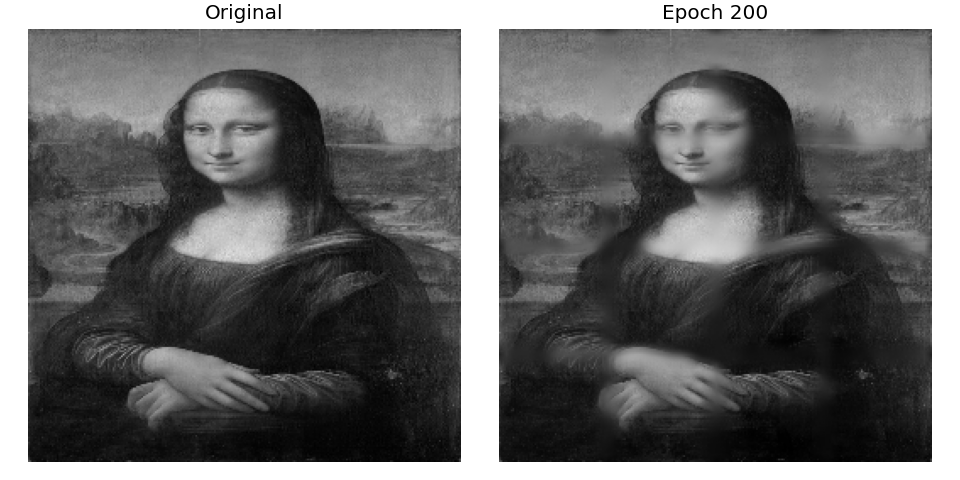
\includegraphics[width=\linewidth]{Main2/outputs/training_analysis/phase_transition_frames/epoch_0200.png}
\end{minipage}
\caption{Static final-epoch reconstruction snapshots for the 1D HVK and 2D HVK experiments. Static epoch frames are used for manuscript reporting instead of animated media.}
\label{fig:final_epoch_frames}
\end{figure}

\section{Discussion}

The experiments show that HVK functions as a hybrid quantum-classical autoencoding framework in which tensor-network patch features provide a compact quantum-inspired representation, positional encoding restores spatial awareness, and the Hamiltonian term guides the latent state toward physically structured correlations. The 1D HVK demonstrates the baseline anisotropic Heisenberg formulation on a one-dimensional chain. The 2D HVK improves the spatial inductive bias by replacing the chain with a two-dimensional qubit grid, allowing horizontal and vertical patch-like correlations to be represented directly.

The key methodological contribution is not the use of MPS, positional encoding, or Hamiltonian optimization independently, but their combination into a single reconstruction architecture. The MPS layer compresses local visual structure, the variational circuit transforms this structure into a symmetry-constrained observable manifold, and the Hamiltonian loss acts as a learned physical prior. The phase-transition analysis gives an interpretable training diagnostic: it identifies epochs where the observable manifold reorganizes sharply, which coincides with the qualitative emergence of coherent reconstructions.

\section{Conclusion}

The recent 1D HVK and 2D HVK outputs support the interpretation that observables shaped by a Hamiltonian loss can serve as a structured latent space for image reconstruction. The 1D HVK validates the one-dimensional Heisenberg formulation and produces high-quality reconstructions with measurable order-parameter dynamics. The 2D HVK extends the method to a two-dimensional interaction graph and achieves the stronger reconstruction benchmark on the present dataset. These results motivate further experiments on larger image collections, multiple benchmark datasets, and direct comparisons against classical autoencoders and quantum autoencoder baselines.

\begin{thebibliography}{9}

\bibitem{krizhevsky2009learning}
A.~Krizhevsky.
\newblock Learning Multiple Layers of Features from Tiny Images.
\newblock Technical report, University of Toronto, 2009.

\end{thebibliography}

\end{document}
